\section{Specifications of the Robot Arm}
\label{sec:spec}

It's necessary to verify the Fanuc LR Mate 200i specifications before any work on the RobWork plugins can commence, because the robot in the laboratory is a LR Mate 200iB and in RobWork it's a LR Mate200iC model. It is essential that the LR Mate model in RobWork is true to the real robot in the laboratory. The model in RobWork (LR Mate200iC) is depicted in the figure below left and the model in the laboratory (LR Mate200iB) is depicted below right. As can be seen from the figure, the models in some points are different however in other cases they are similar.

\begin{figure}[H]
  \centering
  \includegraphics[scale= 0.8]{source/fanucModelPhoto.png}
  \caption{Fanuc Models, left: LR Mate 200iC, right: LR Mate 200iB}
  \label{fig:FanucModels}
\end{figure}

\begin{figure}[H]
  \centering
  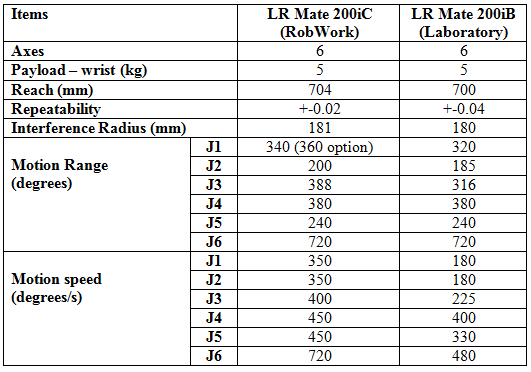
\includegraphics[scale= 0.8]{source/table1.png}
  \caption{Specifications of LR Mate 200iB and LR Mate 200iC}
  \label{fig:tableSpecifications}
\end{figure}

Find the similarity and difference points in the table above from which an analyze can be commenced. As can be seen the main point to analyze is the motion range that is a little bit different between the two models. But physically are the two robots similar with respect to physical length of the joint arms, it's important to get a correct physical representation of the robot in RobWorkStudio. Other points from the table are not so important for use, among this is payload, reach or motion speed, because they are more related to efficiency.

\subsection{Dimensions of the two Models}
By analyzing the datasheet of the two models it can be concluded that the physical appearance of the two Fanuc robots are similar in dimensions. They have six revoloute joints and similar joint arm dimensions. Both models are depicted in the figure \ref{fig:FanucModels}. 
Then DH-parameters can be determined using the datasheet and physically inspecting the robot in the laboratory to verify the dimensions.

\begin{figure}[H]
  \centering
  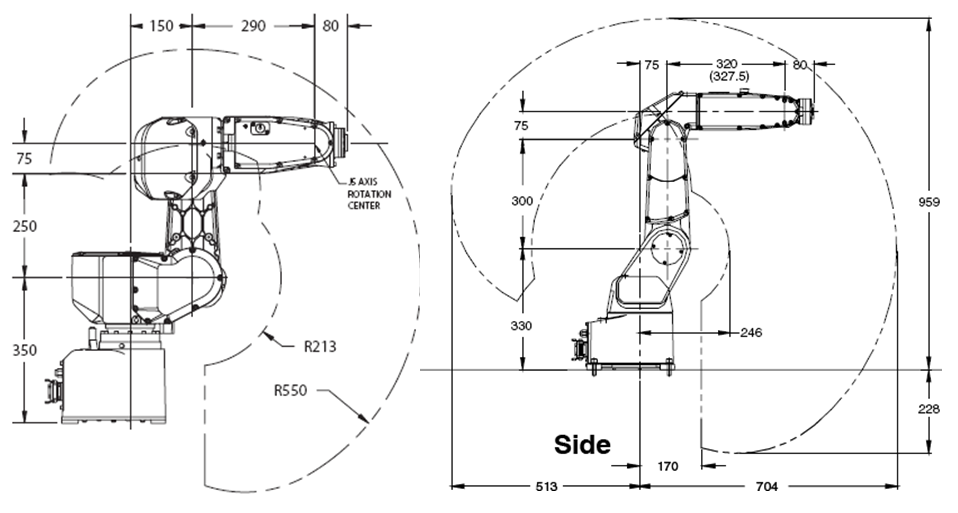
\includegraphics[scale= 0.45]{source/ModelsDimensions.png}
  \caption{left: LR Mate 200iB (Laboratory), right: LR Mate 200iC (RobWork)}
  \label{fig:ModelsDimensions}
\end{figure}

Before determining the DH-parameters, it's important to understand what the meaning of the parameters are, they are defined below:


$a_{i-1} - \text{alpha is angle between } Z_{i} \text{and } Z_{i+1} \text{which is measured about axis }X_{i}\\
a_{i-1} - \text{here distance in mm from  } Z_{i} \text{and } Z_{i+1} \text{which is measured about axis }X_{i}\\
d_{i} - \text{distance from } X_{i-1} \text{to } X_{i} \text{measured along axis  }Z_{i}\\
\theta _{i} - \text{theta is angle between  } X_{i-1} \text{and } X_{i} \text{measured along axis  }Z_{i}$\\

To determine the DH-parameters we need to know the dimensions of both the models, they are shown in the figure \ref{fig:ModelsDimensions}. At the left LR Mate 200iB model which we use in the laboratory and on the right LR Mate 200iC model which we use only to simulate. The determined parameters are shown in the figure \ref{fig:tableParameters}. 

\begin{figure}[H]
  \centering
  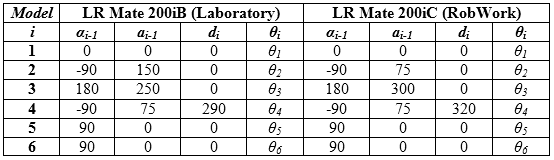
\includegraphics[scale= 0.8]{source/table2.png}
  \caption{DH parameters of LR Mate 200iB and LR Mate 200iC}
  \label{fig:tableParameters}
\end{figure}

From figure\ref{fig:tableParameters} it can be seen that the real model and the model which will be used for simulations is quite similar, however some links are different. However differences are not huge so a decision was made that the model can be used for simulation. The LR Mate 200iB was constructed by using some frames from and the some 3D model objects of the LR Mate 200iC. The model seen in RobWorkStudio are a mix of LR Mate 200iC and LR Mate 200iB, but the dimensions and DH-parameters are determined from the robot in the laboratory.

\subsection{Construction of the Cage}
After verification of the details, measuring the dimensions of where the robot is fixed were made. The LR Mate 200iB stands in the cage as shown in the figure \ref{fig:robworkCage} (here is LR Mate 200iC model). Dimensions of the cage measured and depicted by the RobWorkStudio were created using the XML file. Robot hand stands on the table and around the robot hand is a cage which guarantees the safety of the operator. Position of the LR Mate 200iB in the cage is in the left up corner (if watched from the front view).

\begin{figure}[H]
  \centering
  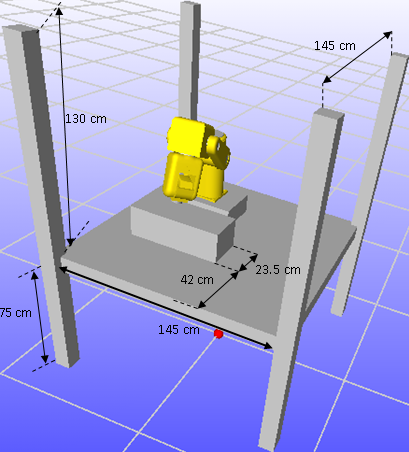
\includegraphics[scale= 0.7]{source/robworkCage.png}
  \caption{Front view of the LR Mate 200i}
  \label{fig:robworkCage}
\end{figure}

Figure \ref{fig:robworkCageDimensions} shows the robot position from top view and dimensions of the cage where LR Mate 200i stands. As can be seen the shape of the table is square, the real table width is a little bit bigger. A smaller is used because it makes it easier to avoid any damage to the cage. A defined smaller work space gives more safety.\newline

Lengths were measured by using the 50 cm ruler. Of course a bigger one would have been better, so there are probably some errors in the measurements $\pm$ 2.5 cm. It's not guaranteed that all values are precise enough.

\begin{figure}[H]
  \centering
  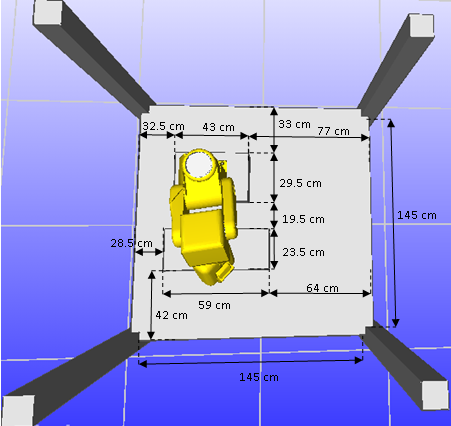
\includegraphics[scale= 0.7]{source/robworkCageDimensions.png}
  \caption{Top view of the LR Mate 200i}
  \label{fig:robworkCageDimensions}
\end{figure}

Regarding this, max theta angles can be determined. They will limit the movements of the joints. If this is not done, there is a risk in damaging the cage or robot.

\subsection{Construction of Joint Angles}
Joint angles means the interval of turning between min and max. By default values were set as shown in the figure \ref{fig:angleDefaultXML}, however a change of those do guarantees that the robot hand can't move too much. If these values are allowed and something is wrong in the state sequence there could be a risk of damage to the window, robot or even worse injure people around. So that is why a desicion was made to limit the turning angle of the robot. 

\begin{figure}[H]
  \centering
  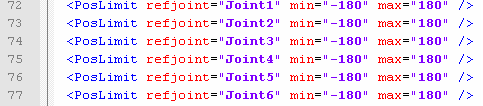
\includegraphics[scale= 0.8]{source/angleDefaultXML.png}
  \caption{Description of LR Mate 200i in Xml (by default)}
  \label{fig:angleDefaultXML}
\end{figure}

Before start an illustration of the robots position in the cage is needed to show all measured dimensions. With all dimensions and joint positions determined, modeling of the turning angles of joint arms could be done. In the XML file each joint has min and max and is set by $\theta _{min}$ and $\theta _{max}$ here theta is angle limits of turning.

\begin{figure}[H]
  \centering
  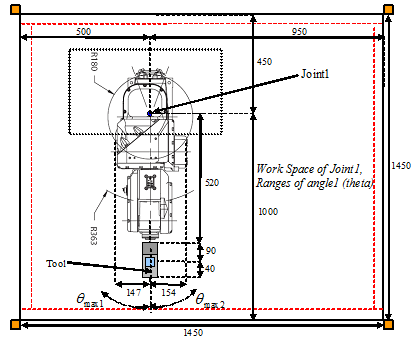
\includegraphics[scale= 1]{source/JointWorkspaceDimensions.png}
  \caption{Work space of Joint1 (Top View)}
  \label{fig:JointWorkspaceDimensions}
\end{figure}

According to figure \ref{fig:JointWorkspaceDimensions} max movements or angles of joint1 can be calculated: \\


$\theta _{min}=\theta _{max1}\\
\theta _{max}=\theta _{max2}$

\begin{align}
\theta _{max1}=arctan\left ( \frac{500-x}{520+90+40} \right ) \label{eq:eq0}\\
\theta _{max2}=\frac{\pi }{2}+arctan\left ( \frac{500-x}{520+90+40} \right )\label{eq:eq1}
\end{align}

In equation 1 the value x is wrong. Depending on the shape of the robot x $>$ 154 is used, x = 180 were chosen. Than max movement range of the joint 1 could be calculated:

$\theta _{max1}=arctan\left ( \frac{500-180}{520+90+40} \right )=arctan\left ( \frac{320}{650} \right )\approx 26deg \\
\theta _{max1}=\frac{\pi }{2}+arctan\left ( \frac{500-180}{520+90+40} \right )=\frac{\pi }{2}+arctan\left ( \frac{320}{650} \right )\approx 116deg$\\


Angles of theta can be illustrated from another view (view from left). Using formula 1 other angles can also be calculated, however we not all of them can be calculated, because the joints are dependent of each other and the here the model is only static. 

\begin{figure}[H]
  \centering
  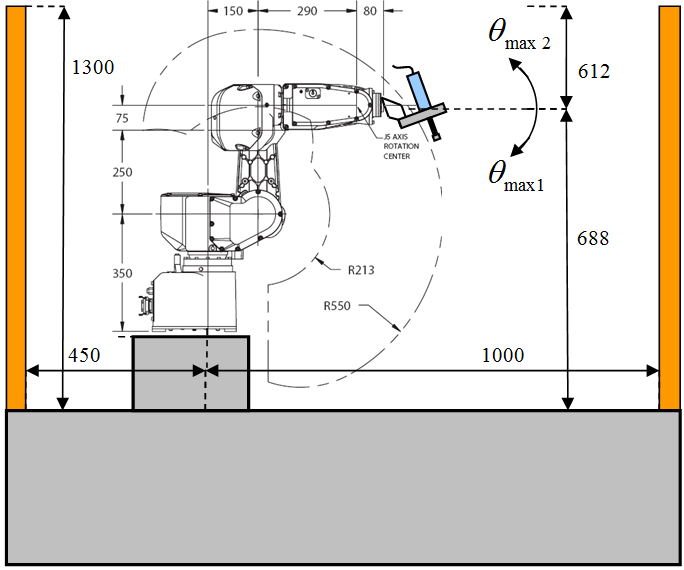
\includegraphics[scale= 0.6]{source/JointWorkspace.png}
  \caption{Work space (Left View)}
  \label{fig:JointWorkspace}
\end{figure}

The chosen calculated angles are shown in the figure \ref{fig:angleXML}. As can be seen, the angles are much smaller than they can be, because of the safety. 

\begin{figure}[H]
  \centering
  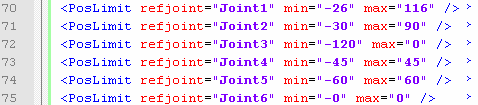
\includegraphics[scale= 0.8]{source/angleXML.png}
  \caption{Description of LR Mate 200i in Xml}
  \label{fig:angleXML}
\end{figure}

\subsection {Modeling the Tool Frame}

Requirement was to have few parameters which let us easily calibrate the tool frame (drill frame). Before that we need to measure the drill which shown in the figure \ref{fig:drillDimensions} (not very nice). As we see from the figure \ref{fig:drillDimensions}, there are two unknowns a and b. Values of a and b let define the position of the drill. As we see than we changing b than we can shift to right or left and it depends mostly of the drill construction. Second one called a is height control of the drill and it possibly changed many times. For instance if we broken the drill or changed the new one. 

\begin{figure}[H]
  \centering
  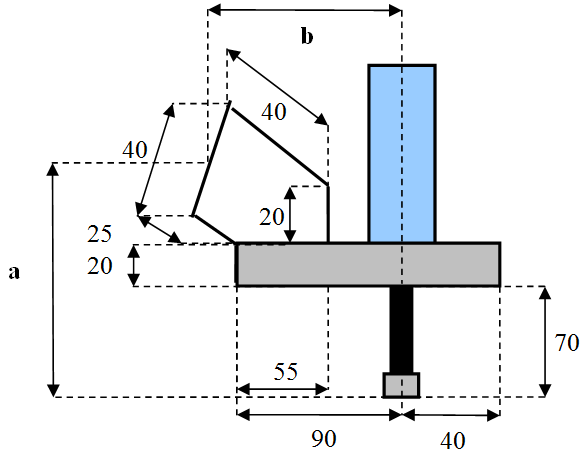
\includegraphics[scale= 0.6]{source/drillDimensions.png}
  \caption{Dimensions of the drill (Tool)}
  \label{fig:drillDimensions}
\end{figure}

Setting of the tool frame were done through an intermediate tool frame. The intermediate tool frame rotates the frame by 45 degrees, because of the drill construction.  Then it's easily to calibrate the tool frame according to the created intermediate frame. As shown in the figure \ref{fig:toolCalibrationXML} there are two values a and b (for more details look at the figure \ref{fig:drillDimensions}) value b is the width of where drill stand and value a is height of the drill.

\begin{figure}[H]
  \centering
  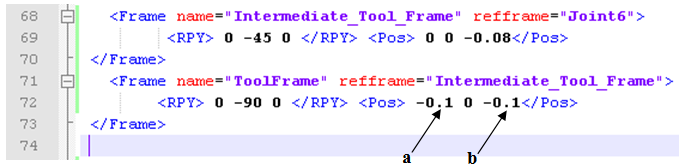
\includegraphics[scale= 0.6]{source/toolCalibrationXML.png}
  \caption{Dimensions of the drill (Tool)}
  \label{fig:toolCalibrationXML}
\end{figure}

The result of the intermediate tool frame and tool frames are shown in the figure \ref{fig:toolFrame}. Configuration of it is shown in the XML file extract (figure \ref{fig:toolCalibrationXML}). Using this any desired tool can easily be used. For instance if a longer drill or a tool with different dimensions than the XML file can be easily modified.

\begin{figure}[H]
  \centering
  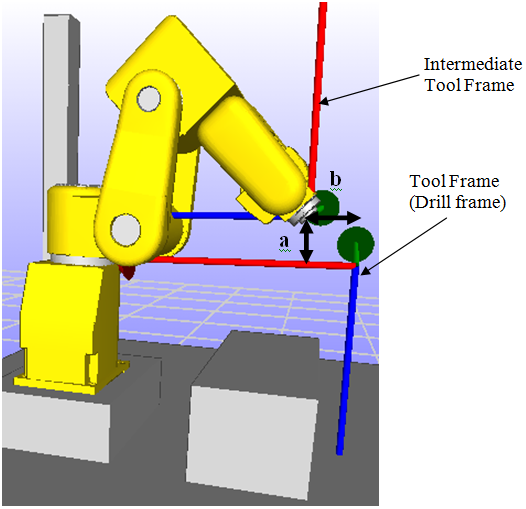
\includegraphics[scale= 0.6]{source/toolFrame.png}
  \caption{Tool frame (drill frame)}
  \label{fig:toolFrame}
\end{figure}

As we can see from the figure \ref{fig:toolFrame} tool frame can be easily modified. Tool frame is important for the future parts, like path planner. Path planner takes Cartesian coordinates from the letter model and moves tool frame regarding it. By moving tool frame all join values change and we need to parse them and send to real robot, but this discussion is out of this chapter scope.

\subsection{Construction of XML File}

Xml file were constructed considering to the few of the things:
\begin{enumerate}
\item Base frame setup. Discussion where set the base frame. It chosen to put center down of the table (cage).
\item Dimensions of the cage. All dimensions were measured and shown in the chapter: "Construction of the cage". Regarding this XML file has parameters which depict the cage.
\item Dimensions of the LR Mate 200iB. Regarding of dimensions were constructed all joints in the XML file.
\item Model graphics of the LR Mate 200iC. Regarding this was used 3D model to illustrate simulate robot behavior.
\item Collision setup. There was added reference to collision setup which indicates collisions of the LR Mate 200iC model.
\end{enumerate} 

\subsection{Construction of Joints}
LR Mate 200iB has six axes. Each axis is revolute, dimensions given by manufacturer. Regarding this we can start to create joints in XML. We can do by two ways:
\begin{enumerate}
\item Calculate positions of the joints by using template of the Fanuc 200i model. This was given by RobWork, however model is not quite the same.
\item Calculate DH parameters and regarding this construct the XML file with joints
\end{enumerate} 

We use first approach because in the assignment there was no appointment how to construct. First approach was used for someone but parameters were not the same, so we need to recalculate all parameters. Before start to construct the joints we need to define where put a base frame. From the base frame all other joints will be constructed. There were discussions where to put the base frame. One opinion was to put base frame at the one of the table corners, another one where robot centre stands and last one down centre of the table. We decided to choose last one, because there was easiest way to start construct table and after that joints. Reason was that the base frame will stand independently to any of the objects around it.
Second approach will be more useful, reason of easier understand and adopt new changes of the robot. For instance if the lengths Robot arm changed. We actually need change DH parameters in the XML by entering into places like shown in the figure \ref{fig:DHParameters}. 

\begin{figure}[H]
  \centering
  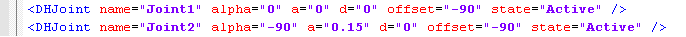
\includegraphics[scale= 0.65]{source/DHParameters.png}
  \caption{Example of configuration by DH parameters}
  \label{fig:DHParameters}
\end{figure}




